\documentclass[10pt, a4paper]{article}

\usepackage[utf8]{inputenc}
\usepackage[spanish]{babel}
\usepackage{graphicx}
\usepackage{multicol}
\usepackage[usenames,dvipsnames]{color}
\usepackage{amsmath}
\usepackage{verbatim}
\usepackage{footnote}
\usepackage{float}
\usepackage{amsfonts}
\usepackage{hyperref}
\usepackage{framed}
\usepackage{multicol}
\usepackage{pdflscape}

\usepackage{pdfpages}

\usepackage{caratula}

\newcommand{\NonStandardConector}[2] {
	\item \textbf{#1} : #2
}

\materia{Ingeniería de Software II}

\titulo{Trabajo Práctico 2}
\subtitulo{Developing \textsf{in-the-large} - Planificación}
\grupo{Grupo 5 - \emph{El nene está bien}}

\integrante{Martín Alejandro Miguel}{181/09}{m2.march@gmail.com}
\integrante{Iván Postolski}{216/09}{ivan.postolski@gmail.com}
\integrante{Juan Manuel Martinez Caamaño}{276/09}{jmartinezcaamao@gmail.com}
\integrante{Matías Incem}{396/09}{matias.incem@gmail.com}
\integrante{Pablo Gauna}{334/09}{gaunapablo@gmail.com}

\setcounter{tocdepth}{2}

\begin{document}

\maketitle
\tableofcontents
\newpage

\section{Introducción}

	Para este trabajo practico se nos pide planificar y diagramar la arquitectura de una aplicación para ahorradores. Esta aplicación, de forma similar a \emph{Precio Justo} (presentada en el primer trabajo practico), deberá servir para que ahorradores puedan consultar a través por ofertas, de distintos productos, publicadas en distintas redes sociales y medios de internet. Sin embargo, a diferencia de \emph{Precio Justo}, el alcance de esta aplicación resulta ser mucho mayor. 

Para esta entrega se nos pide:
\begin{enumerate}
	\item \emph{Atributos de calidad} identificadas en la situación planteada, presentado en la sección \ref{sec:calidad}.
	\item Diagrama de la \emph{arquitectura}, en la seccion \ref{sec:arquitectura}. Ademas, se explica como esta satisface los atributos de calidad, planteados en esta entrega, y los casos de uso introducidos en la entrega anterior.
	\item Comparación entre \emph{Unified Process} y \emph{Scrum}, y comparación entre \emph{Programming in the small} con \emph{Programming in the large}. Esto ultimo se detalla en la sección \ref{sec:comparacion}.
\end{enumerate}

Adicionalmente en la sección \ref{sec:cu}, los casos de uso de la entrega anterior son recordados.


\section{Atributos de calidad}
	\label{sec:calidad}

	\begin{itemize}
\item
  \emph{Extensibilidad} de las fuentes de datos. (2do párrafo enunciado)

  \begin{itemize}
  \item
    Fuente: El equipo de desarrolladores.
  \item
    Estimulo: Se desea implementar una nueva fuente de datos.
  \item
    Artefacto: Sistema de obtención de datos.
  \item
    Entorno: En funcionamiento normal.
  \item
    Respuesta: Se implementa la fuente de datos y se la integra al
    sistema.
  \item
    Medida: La fuente de datos se integra con el sistema en menos de 1
    hora, sin detener al sistema.
  \end{itemize}
\item
  \emph{Modificabilidad} de los bots que obtienen datos.

  \begin{itemize}
  \item
    Fuente: El equipo de desarrolladores.
  \item
    Estimulo: Se desea implementar/modificar/eliminar un bot para
    obtener datos de una pagina web determinada.
  \item
    Artefacto: Sistema de obtención de datos.
  \item
    Entorno: En funcionamiento normal.
  \item
    Respuesta: Se implementa el bot y se integra con el sistema.
  \item
    Medida: el bot se implementa o modifica en menos de 25 horas y se
    integra con el sistema en menos de 1 hora, sin detener al sistema.
  \end{itemize}
\item
  \emph{Detección de fallas} en la información obtenida por los bots.

  \begin{itemize}
  \item
    Fuente: Las paginas monitoreadas.
  \item
    Estimulo: Se produce un cambio en la estructura de las paginas
    monitoreadas.
  \item
    Artefacto: Bot del sistema de obtención de datos.
  \item
    Entorno: En funcionamiento normal.
  \item
    Respuesta: Se detecta el cambio en la estructura de la pagina, se
    detiene el bot, y se informa a los administradores.
  \item
    Medida: Cuando de una serie de consultas, se detecta un 70\% de
    cambios en su estructura, se considera como error.
  \end{itemize}
\item
  \emph{Modificabilidad} de los rubros y productos de rubros. (3pe)

  \begin{itemize}
  \item
    Fuente: Administradores del sistema.
  \item
    Estimulo: Se desea agregar un nuevo producto/rubro.
  \item
    Artefacto: Sistema central TPA.
  \item
    Entorno: Funcionamiento normal.
  \item
    Respuesta: Utilizando la interfaz de administración, se agrega un
    nuevo producto/rubro al sistema, sin detenerlo.
  \item
    Medida: Se agrega un producto/rubro en menos de 5 minutos.
  \end{itemize}
\item
  \emph{Modificabilidad} de las reglas de asociación y sustitución.
  (3pe)

  \begin{itemize}
  \item
    Fuente: Administradores del sistema
  \item
    Estimulo: Se desea agregar/modificar las reglas de asociación y
    sustitución.
  \item
    Artefacto: Sistema central TPA.
  \item
    Entorno: Modo de mantenimiento.
  \item
    Respuesta: Se modifican las reglas de asociación y sustitución.
  \item
    Medida: En menos de 24hs se implementan y ponen en funcionamiento
    las modificaciones a estas reglas.
  \end{itemize}
\item
  \emph{Performance} para velocidad en que se identifican ofertas de las
  distintas fuentes de datos. (4pe)

  \begin{itemize}
  \item
    Fuente: Usuario externo
  \item
    Estimulo: Se publica en un medio monitoreado por el sistema de
    obtención de datos una oferta.
  \item
    Artefacto: Sistema de obtención de datos.
  \item
    Entorno: Funcionamiento normal.
  \item
    Respuesta: El sistema de obtención de datos identifica esta oferta y
    la agrega a la base de datos.
  \item
    Medida: La oferta se comienza a tener en cuenta 10 segundos despues
    de que fue publicada por una fuente de datos.
  \end{itemize}
\item
  \emph{Usabilidad}, sistema de confianza facilmente configurable.

  \begin{itemize}
  \item
    Fuente: Usuario autentificado.
  \item
    Estimulo: Modifica las reglas de confianza de ofertas.
  \item
    Artefacto: Sistema central TPA.
  \item
    Entorno: Funcionamiento normal.
  \item
    Respuesta: Se modifican las reglas de confianza de ofertas.
  \item
    Medida: El sistema provee una guia de configuración de confianza de
    ofertas, que ayuda a completar dicha tarea en menos de 15 minutos
    para un usuario nuevo.
  \end{itemize}
\item
  \emph{Extensibilidad} de las fuentes de confianza de datos del
  usuario.

  \begin{itemize}
  \item
    Fuente: Equipo de desarrollo.
  \item
    Estimulo: Se desea agregar una nueva fuente de confianza de datos
    del usuario.
  \item
    Artefacto: Sistema central TPA.
  \item
    Entorno: Modo de mantenimiento.
  \item
    Respuesta: Se agrega la fuente de confianza de datos al sistema.
  \item
    Medida: La fuente de confianza se implementa en menos de 25hs y se
    integra al sistema en menos de 1 hora.
  \end{itemize}
\item
  \emph{Modificabilidad} del servicio de deteccion de spam.

  \begin{itemize}
  \item
    Fuente: Equipo de desarrollo.
  \item
    Estimulo: Se desea modificar el funcionamiento del servicio de
    detección de Spam.
  \item
    Artefacto: Sistema de detección de Spam.
  \item
    Entorno: Funcionamiento normal.
  \item
    Respuesta: Se modifica el funcionamiento del servicio.
  \item
    Medida: El funcionamiento del servicio de detección de Spam debe
    poder modificarse (Cambio de proveedor, nuevo proveedor,
    etc\ldots{}) con el sistema en funcionamiento Normal, y deberia ser
    posible que mas de un sistema de detección de Spam puedan
    co-existir.
  \end{itemize}
\item
  \emph{Auditabilidad} para ver la cantidad de ofertas falsas
  detectadas, productos de precios dudosos, etc.

  \begin{itemize}
  \item
    Fuente: Administradores del sistema.
  \item
    Estimulo: Se desea ver el resumen de ofertas falsas, detectadas,
    etc\ldots{}
  \item
    Artefacto: Sistema de detección de Spam.
  \item
    Entorno: Funcionamiento normal.
  \item
    Respuesta: Se obtiene un resumen con la información de ofertas
    falsas detectadas, precios dudosos, etc\ldots{}
  \item
    Medida: Cada vez que se elimina / modifica una oferta se registra
    `quien, cuando, por que (precio dudoso, oferta falsa, etc\ldots{}),
    y la oferta'.
  \end{itemize}
\item
  \emph{Usabilidad} de la interfaz del sistema para realizar consultas.

  \begin{itemize}
  \item
    Fuente: Un usuario nuevo.
  \item
    Estimulo: El usuario desea realizar una consulta.
  \item
    Artefacto: Interfaz Movil / Interfaz Web.
  \item
    Entorno: Funcionamiento normal.
  \item
    Respuesta: Se realiza la consulta y se informa de los resultados a
    los usuarios.
  \item
    Medida: En menos de 5 minutos, un usuario nuevo comprende la
    interfaz y comienza a utilizarla .
  \end{itemize}
\item
  \emph{Usabilidad} de la interfaz del sistema mientras se realizan
  consultas.

  \begin{itemize}
  \item
    Fuente: Un usuario.
  \item
    Estimulo: El usuario desea realizar una consulta.
  \item
    Artefacto: Interfaz Movil / Interfaz Web.
  \item
    Entorno: Funcionamiento normal.
  \item
    Respuesta: Conforme se escribe la respuesta, se muestran resultados.
  \item
    Medida: En menos de 1 segundo luego de que se comenzo a tipear una
    consulta, el sistema comienza a sugerir posibles resultados.
  \end{itemize}
\item
  \emph{Usabilidad} de la interfaz del sistema, antes de realizar
  consultas.

  \begin{itemize}
  \item
    Fuente: Un usuario.
  \item
    Estimulo: Se accede a la interfaz y aun no se realiza ningun tipo de
    consulta.
  \item
    Artefacto: Interfaz Movil / Interfaz Web.
  \item
    Entorno: Funcionamiento normal.
  \item
    Respuesta: Se comienzan a presentar resultados.
  \item
    Medida: Se muestran las ofertas populares / mas buscadas / mas
    recomendadas.
  \end{itemize}
\item
  \emph{Disponibilidad} del servicio.

  \begin{itemize}
  \item
    Fuente: Usuario.
  \item
    Estimulo: Se desea realizar una consulta.
  \item
    Artefacto: Interfaz movil.
  \item
    Entorno: Funcionamiento normal.
  \item
    Respuesta: Se realiza la consulta al sistema, se obtienen resultados
    y son mostrados al usuario.
  \item
    Medida: En el 99\% de los casos la consulta se realiza con exito al
    sistema central.
  \end{itemize}
\item
  \emph{Disponibilidad} del servicio cuando no hay conección.

  \begin{itemize}
  \item
    Fuente: Usuario.
  \item
    Estimulo: Se desea realizar una consulta.
  \item
    Artefacto: Interfaz movil.
  \item
    Entorno: Funcionamiento sin conección
  \item
    Respuesta: Si la consulta se encuentra disponible sin conección, se
    obtienen los resultados y son mostrados al usuario.
  \item
    Medida: Las ultimas consultas y las consultas mas populares al
    momento de la ultima conección se encuentran disponibles.
  \end{itemize}
\end{itemize}


\section{Arquitectura}
	\label{sec:arquitectura}

\subsection{Referencia de conectores}
A continuación presentamos una referencia a los conectores utilizados en los diagramas que se presentaran en las siguientes secciones. Los conectores \emph{no-standard} utlizados son especificados mas abajo.

\begin{figure}[H]
	\centering
	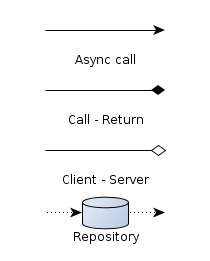
\includegraphics[scale=0.6]{graficos/call_reference.png}
	\caption{Referencia de conectores.}
\end{figure}

\subsubsection{Conectores no estandar}

\begin{itemize}
		%Completar con conectores no standard!
		%Agregar asi:
		\NonStandardConector{A non standard conector name}{A non standard conector description.}
\end{itemize}

\subsection{Subsistema de Query}

En el siguiente diagrama presenta el \textsf{Subsistema de Query} donde dada una consulta por productos (\textbf{query}) se arma la respuesta al usuario que realizó la consulta. En este diagrama se encuentran ejemplificados los \emph{casos de uso} 7, 8, 9, 10, 11 y 12.

\begin{figure}[H]
	\centering
	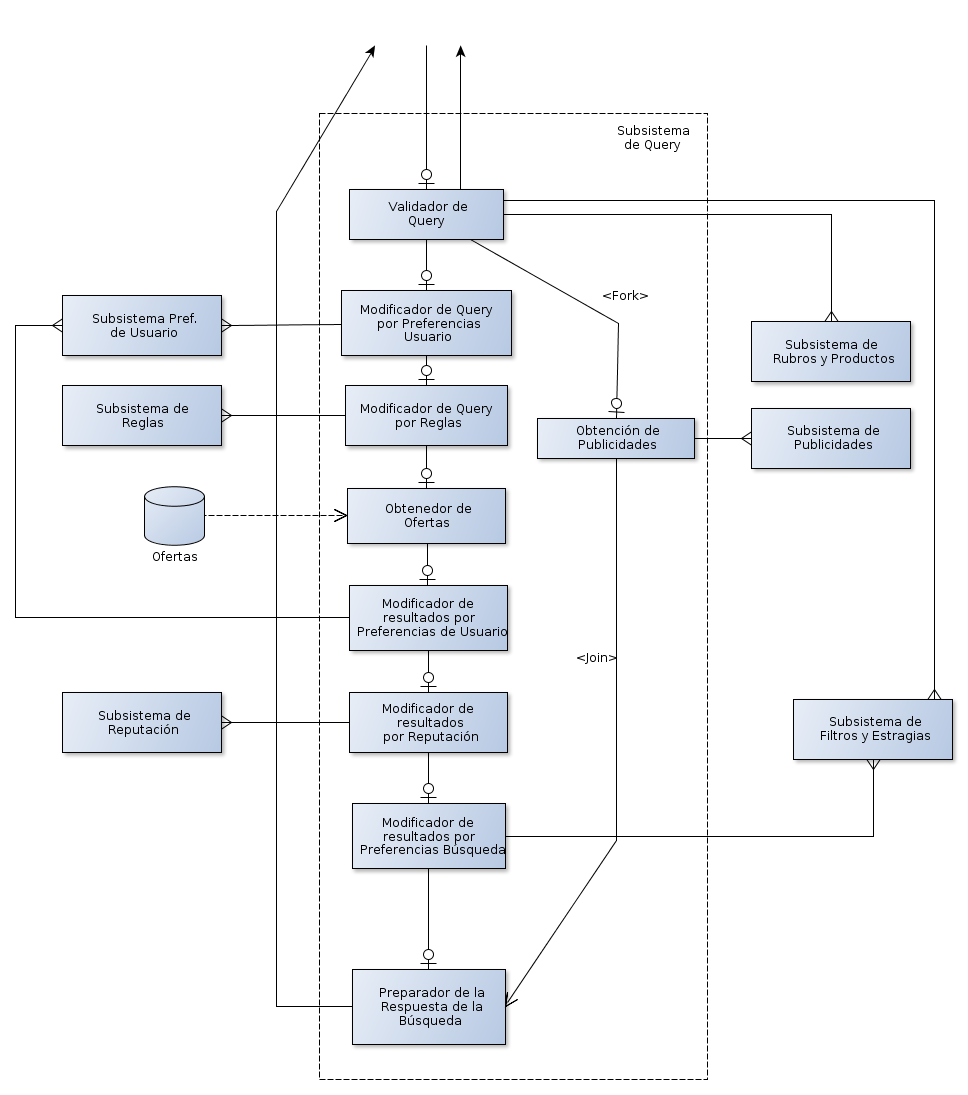
\includegraphics[width=\textwidth]{graficos/arch/subsistema_query.png}
	\caption{Diagrama arquitectónico con el detalle del \textsf{Subsistema de Query}.}
\end{figure}

\subsection{Interfaz movil}

\begin{figure}[H]
	\centering
	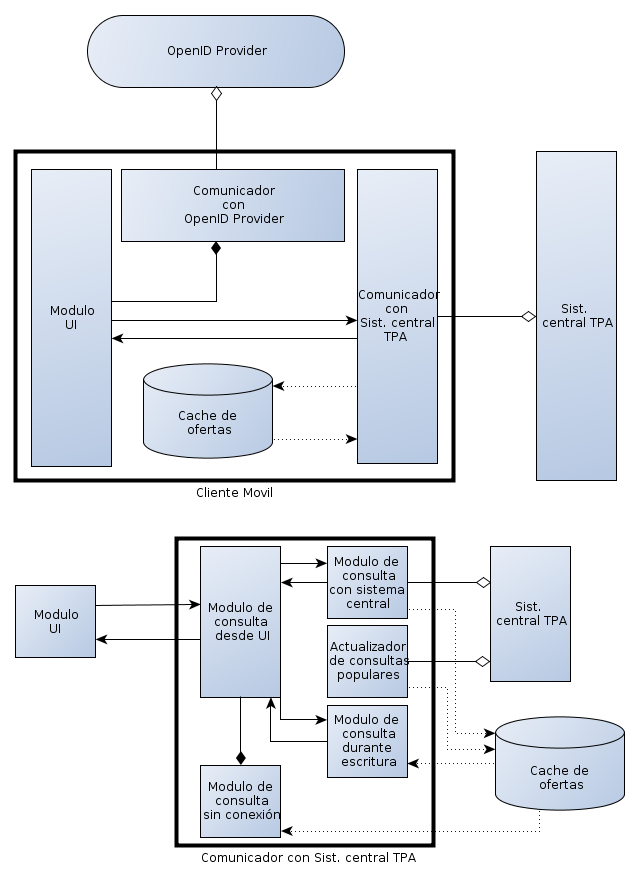
\includegraphics[width=\textwidth]{graficos/arch/Cliente_movil.png}
	\caption{Diagrama arquitectónico con el detalle del \textsf{Cliente movil}.}
\end{figure}


\section{Comparación}
	\label{sec:comparacion}

	\subsection{Comparación Metodologias agiles y Unified Process}

	Tanto \emph{Unified Process} como \emph{Scrum} son metodologias para el desarrollo de software, estas proponen un marco de trabajo para planificar y controlar distintas etapas en el desarrollo de software.

	Una caracteristica comun en ambas metodologias, es que siguen un proceso \emph{iterativo incremental}. Esto quiere decir que en ambas metodologias, el desarrollo del software se realiza en forma de iteraciones bien definidas. Una de las principales diferencias, encontradas durante la realización de los trabajos practicos de la materia, es que Unified Process organiza el desarrollo de software en distintas \emph{etapas} (\emph{inception, elaboration, construction} y \emph{transition}), cada etapa se diferencia de las otras en la actividad sobre la cual se pone enfasis. Sin embargo, en cada etapa se podrian realizar cada una de las posibles actividades (desarrollo, requerimientos, testing, etc...). Por otro lado, metodologias agiles como Scrum, no establecen nignuna distinción de etapas en el desarrollo.

	Esto se refleja en que para desarrollar la aplicación \emph{Precio Justo}, se partio de una escasa planeación sobre la construcción del software a desarrollar, en cambio, para \emph{Twitteando para ahorrar} se parte de un \emph{plan de iteraciones} y de una \emph{elaboración de la arquitectura} bien definida y documentada (si bien este plan y la arquitectura pueden estar sujetos a cambios).

	El desarrollo en Scrum, se centra en priorizar las funcionalidades que otorguen mas 'valor' al producto, esto se refleja en la idea de organizar las tareas a realizar en cada iteración en \emph{user stories}, una serie de historias, similares a casos de uso, contadas desde el punto de vista del usuario/product owner de la aplicación. En cambio, en Unified Process, las tareas a realizar en cada iteración estan son elegidas con el objetivo de reducir los riesgos. Para capturar las funcionalidades a implementar en cada iteración, Unified Process utiliza \emph{casos de uso}.

	De tener que escoger una metodologia para el desarrollo de software, nosotros creemos que \textbf{no} tiene sentido elegir de forma \emph{estricta} una unica metodologia. Nosotros proponemos utilizar ambas metodologias como un marco de ideas para construir una metodologia que se adapte de la mejor forma a nuestro equipo y al proyecto con el cual nos enfrentemos.
	De ambas metodologias, las caracteristicas que mas nos gustaron son:

	\begin{itemize}
		\item En este momento, Juan esta QUE-MA-DO.
	\end{itemize}

\subsection{Comparación 'programming in the small' y 'programming in the large'}



\section{Casos de uso}
	\label{sec:cu}

	\subsubsection{CU1: Obteniendo informacion de internet}

\textbf{Descripción}: El sistema colecta la información de los distintos
medios, la procesa, y la almacena para luego ser provista a los
usuarios.

\subsubsection{CU2: Se consulta información a travéz de el API publica.}

\textbf{Descripción}: Clientes externos pueden consultar a nuestro
sistema por precios que recopilamos de distintos medios a través de un
servicio público (API) ofrecido por nuestro sistema.

\subsubsection{CU3: El usuario consulta precios a través de una interfaz
amigable}

\textbf{Descripción}: El usuario accede a una aplicación de celular
propia de \emph{twitteando para ahorrar} a través de la cual puede
consultar por precios para distintos productos.

\subsubsection{CU4: Se realizó una consulta por un producto, y el
dispositivo sin tener conexión, logra responder la consulta de alguna
forma medianamente satisfactoria.}

\textbf{Descripción}: El usuario accede a la aplicación de celular
\emph{twitteando para ahorrar} sin tener conectividad a internet y
recibe precios de los productos deseados y los relacionados a estos. La
información provista al usuario podría estar limitada respecto de lo que
vería si tuviera conectividad, pero esto no debería ser notado por el
mismo.

\subsubsection{CU5: ABM de rubros habilitados.}

\textbf{Descripción}: Ciertos usuarios particulares del sistema pueden
acceder al mismo para agregar nuevos rubros o modificar o borrar
existentes.

\subsubsection{CU6: ABM de productos en un rubro.}

\textbf{Descripción}: Ciertos usuarios particulares del sistema pueden
acceder al mismo para agregar nuevos productosi o modificar o borrar
existentes. También pueden redefinir la pertenencia de un producto a uno
o más rubros.

\subsubsection{CU7: Si realizo una consulta por un producto A, obtengo
ofertas de este producto.}

\textbf{Descripción}: El usuario consulta por un producto A dentro de
los habilitados en algún rubro y recibe información de donde comprarlo y
a qué precio.

\subsubsection{CU8: Si realizo una consulta por un producto A y este no
está se le informa al usuario.}

\textbf{Descripción}: El usuario consulta por un producto A que no está
habilitado en ningún rubro y es informado que el sistema no posee
información sobre donde comprar el mismo.

\subsubsection{CU9: Si realizo una consulta por un producto A, y se
considera que puede sustituirse por B, tambien se muestran ofertas de
B.}

\textbf{Descripción}: El usuario consulta por un producto A dentro de
los habilitados en algún rubro y se definió que puede sustituirse por el
producto B, luego el usuario recibe información de donde comprar A y
donde comprar B y a qué precio.

\subsubsection{CU10: Si realizo una consulta por un producto A, que se
considera asociado con B, tambien se muestran ofertas de B.}

\textbf{Descripción}: El usuario consulta por un producto A dentro de
los habilitados en algún rubro y se definió que está asociado con el
producto B, luego el usuario recibe información de donde comprar A y
donde comprar B y a qué precio.

\subsubsection{CU11: Si realizo una consulta por un producto A y soy un
usuario autentificado, las ofertas recibidas se priorizan acorde a mis
preferencias de confianza.}

\textbf{Descripción}: Dentro de las ofertas relacionadas al producto A
que conoce el sistema, se mostrarán primero aquellas cuya fuente yo haya
declarado de mayor confianza, luego las de fuentes con menor confianza y
no se mostrará ninguna oferta cuya fuente declaré como no confiable.

\subsubsection{CU12: Mostrando publicidades}

\textbf{Descripción}: Cuando el usuario utiliza la aplicación movil
visualiza, aparte de los resultados de su consulta, propaganda de los
spónsores de \emph{twitteando para ahorrar}.

\subsubsection{CU13: Detectando ofertas falsas}

\textbf{Descripción}: Al recopilar datos de precios en internet, el
sistema es capaz de detectar si la información es sospechosa y marcarla
como tal, para futura revisión. Además el sistema recopila todas las
evidencias encontradas para sospechar de los datos.

\subsubsection{CU14: Siendo martes se publica un informe de ofertas
falsas}

\textbf{Descripción}: Cada martes el sistema arma y publica un informe
con los productos sobre los cuales se encontraron precios dudosos junto
con la evidencia que genera la sospecha. Este informe debe estar
disponible para revisión por usuarios externos selectos.

\subsubsection{CU15: Se prepara un informe con las estadisticas de
ofertas detectadas como falsas.}

\textbf{Descripción}: Al mismo tiempo que el usuario comienza a ingresar
una consulta en la aplicación movil, la aplicación se anticipa a los
deseos del usuario para mostrarle rápidamente precios de productos que
podríán responder a la consulta que se está formulando.

\subsubsection{CU16: El usuario se autentica con el sistema}

\textbf{Descripción}: El usuario de la aplicación movil puede utilizar
alguna cuenta de un servicio asociado con OpenID (google, yahoo,
facebook y otro) para autenticarse en la aplicación. A partir de ese
momento la aplicación sabe quién es el usuario y puede utilizar la
información que tiene del mismo para proveerle funcionalidades más
avanzadas.

\subsubsection{CU17: Un usuario autentificado puede votar por la validez
de una oferta.}

\textbf{Descripción}: Un usuario ya autenticado en el sistema elije una
oferta y la marca como válida o inválida. Esto afecta la reputación del
usuario o fuente que dio origen a la oferta para facilitar la detección
de ofertas sospechosas.


\end{document}
